\documentclass[11pt, a4paper]{article}

% --- Packages ---
\usepackage[utf8]{inputenc}
\usepackage[T1]{fontenc}
\usepackage{mathptmx} % Times New Roman font for professional document typography
\usepackage{graphicx}
\usepackage[margin=0.8in]{geometry}
\usepackage{xcolor}
\usepackage{titlesec}
\usepackage{enumitem}
\usepackage{float}
\usepackage{booktabs}
\usepackage{multirow}
\usepackage{array}
\usepackage{amsmath,amssymb}
\usepackage{hyperref}
\usepackage{subcaption}

\hypersetup{
    colorlinks=true,
    linkcolor=amritaMaroon,
    citecolor=amritaMaroon,
    urlcolor=amritaMaroon
}

% --- Amrita Colors ---
\definecolor{amritaMaroon}{HTML}{A4123F}

% --- Title & Section Formatting ---
\titlespacing*{\section}{0pt}{12pt}{4pt}
\titlespacing*{\subsection}{0pt}{8pt}{3pt}
\titleformat{\section}{\large\bfseries\color{amritaMaroon}}{\thesection}{0.8em}{}
\titleformat{\subsection}{\normalsize\bfseries\color{amritaMaroon}}{\thesubsection}{0.6em}{}

\pagestyle{plain}

\begin{document}

% ==========================================
% HEADER & TITLE BLOCK
% ==========================================
\noindent
\begin{minipage}{\textwidth}
    \centering
    {\Large \textbf{\textcolor{amritaMaroon}{
    AMRITA VISHWA VIDYAPEETHAM \\
    SCHOOL OF COMPUTING \\
    DEPARTMENT OF COMPUTER SCIENCE AND ENGINEERING \\
    }}}
    \vspace{0.2cm}
    {\large \textbf{Explainable Federated Learning for Healthcare Time-Series Forecasting with Personalized Drift Adaptation (FPDAF)}} \\[0.1cm]
    \textbf{23CSE498 -- Project Phase II (External Review)} \quad | \quad \textbf{Team Number: G028} \\
    November 16, 2026
\end{minipage}

\vspace{0.3cm}
\hrule
\vspace{0.3cm}

% --- Team & Guide Details ---
\noindent
\begin{center}
    \renewcommand{\arraystretch}{1.35}
    \setlength{\tabcolsep}{5pt}
    \small
    \begin{tabular}{|l|p{4.6cm}|p{4.4cm}|p{3.0cm}|}
        \hline
        \multicolumn{2}{|c|}{\textbf{Team Members}} & \textbf{Project Guide} & \textbf{Project Type} \\
        \hline
        CB.SC.U4CSE23547 & SHEELA AKSHAR SAKHI (Lead) &
        \multirow{5}{=}{\raggedright \textbf{Dr. G. R. Ramya} \newline \textit{Asst. Professor (Sr. Gr.)} \newline \textbf{Dr. S. Vandhana} \newline \textit{Asst. Professor} \newline Dept. of CSE \newline \textbf{Dr. Pallavi, MD} \newline \textit{Clinical Intensivist}} &
        \multirow{5}{=}{\raggedright \textbf{Type 1} \newline Research-Based Project \newline \textbf{100\% Completed}} \\ \cline{1-2}
        CB.SC.U4CSE23529 & HASINI REDDY M & & \\ \cline{1-2}
        CB.SC.U4CSE23761 & KOUSIK SARMA LAKKARAJU & & \\ \cline{1-2}
        CB.SC.U4CSE23363 & HASWITHA K & & \\ \cline{1-2}
        CB.SC.U4CSE23753 & V. CHAKRAVARTHY & & \\
        \hline
    \end{tabular}
\end{center}
\vspace{0.2cm}

% ==========================================
% 1. ABSTRACT
% ==========================================
\section{Abstract}
\noindent
Sepsis remains the leading cause of in-hospital mortality worldwide, claiming over 11 million lives annually with an hourly therapeutic delay penalty of $7.6\%$--$8.0\%$ in septic shock survival. Although deep learning on high-frequency intensive care unit (ICU) multivariate telemetry enables early onset forecasting, translation into multi-hospital networks is obstructed by three foundational barriers: (1)~\textit{the privacy barrier} imposed by statutory health data regulations (HIPAA, GDPR, and India's DPDPA 2023), (2)~\textit{the accuracy barrier} induced by inter-institutional patient demographic and practice pattern concept drift, and (3)~\textit{the trust barrier} caused by uncalibrated black-box alarms triggering clinical alert fatigue. This project delivers the \textbf{Federated Personalized Drift-Aware Attention Framework (FPDAF)}, a 100\% completed decentralized clinical decision support system. FPDAF integrates a split-weight \texttt{DualPhaseAttentionLSTM} backbone capturing both temporal trajectory and cross-vital co-dependencies, an online \textbf{AD-CUSUM} concept drift detector combining Jensen-Shannon divergence with gradient variance, a \textbf{DDP-ERP} entropy-regularized personalization objective, and a \textbf{CSSP} client-side selective freeze protocol. Benchmarked on $N = 102,994$ strictly patient-disjoint held-out test windows ($6,050$ patients) across three heterogeneous institutional tiers from the PhysioNet 2019 CinC Challenge, FPDAF achieves top precision-recall discrimination ($\text{AUPRC} = 0.1043$, $\text{AUROC} = 0.7923$), superior probability calibration ($\text{ECE} = 0.0902$, $\text{Brier} = 0.0548$), a $63.1\%$ Brier reduction under late-ICU concept drift, a $48.6\%$ communication uplink bandwidth reduction, and a real-time edge inference latency of $0.67\text{ ms}$ on Apple Silicon M4. The framework is fully deployed into an operational 3-tier clinical workstation providing bedside Surviving Sepsis Campaign Hour-1 guidance and axiomatic feature attributions.

% ==========================================
% 2. PROBLEM DEFINITION & LITERATURE REVIEW
% ==========================================
\section{Problem Definition, Research Motivation \& Literature Review}

\subsection{Problem Statement \& Research Motivation}
\begin{itemize}[noitemsep, topsep=2pt]
    \item \textbf{Formal Problem Statement:} Given a decentralized network of $K$ distinct clinical institutions, where each center $k \in \{1, \dots, K\}$ holds a private set of longitudinal ICU patient trajectories $\mathcal{D}_k = \{(X_i, y_i)\}_{i=1}^{N_k}$, with $X_i \in \mathbb{R}^{T \times D}$ representing $T = 24$ hourly observations over $D = 40$ physiological parameters (vital signs, laboratory tests, and demographics), the objective is to collaboratively train an early sepsis forecasting model $\hat{y}_i = f(X_i; \theta)$ that predicts Sepsis-3 clinical onset $6\text{ hours}$ in advance without centralizing patient telemetry $\mathcal{D}_k$, while adapting dynamically to local institutional concept drift and providing clinically calibrated risk probabilities.
    \item \textbf{Clinical Motivation \& Urgency:} Sepsis accounts for 1 in every 5 deaths globally. In critical care units, hemodynamic collapse occurs abruptly. Clinical trial evidence confirms that every hour of delayed antimicrobial therapy following septic shock onset lowers survival probability by approximately $7.6\%$ \cite{kumar2006duration}. Continuous multi-center clinical machine learning offers early warning; however, hospital legal firewalls strictly prohibit centralized data aggregation under HIPAA, GDPR, and DPDPA 2023 regulations.
    \item \textbf{The Three Foundational Healthcare Gaps:}
    \begin{enumerate}[noitemsep, topsep=2pt]
        \item \textit{The Privacy Gap:} Multi-institutional clinical datasets cannot be pooled into a centralized data warehouse due to statutory privacy compliance.
        \item \textit{The Accuracy Gap (Non-IID Drift):} Patient demographics, admission acuity, and lab testing frequencies diverge widely across community hospitals, trauma centers, and geriatric ICUs, creating severe covariate and concept drift that deteriorates naive federated consensus models (e.g., FedAvg).
        \item \textit{The Trust Gap:} Deep models frequently exhibit severe overconfidence in uncalibrated probabilities under class imbalance (sepsis prevalence $\approx 2.5\%$), inducing clinician cynicism and alarm fatigue.
    \end{enumerate}
    \item \textbf{Measurable Research Objectives:}
    \begin{enumerate}[noitemsep, topsep=2pt]
        \item \textit{Objective 1:} Formulate a split-weight federated neural architecture that decouples universal temporal dynamics from institution-specific risk calibration.
        \item \textit{Objective 2:} Develop an online concept drift detection and client-side selective freezing mechanism that absorbs stochastic measurement noise while rapidly triggering local adaptation under real distribution shifts.
        \item \textit{Objective 3:} Achieve superior predictive discrimination ($\text{AUPRC} \ge 0.10$, $\text{AUROC} \ge 0.79$) and probability calibration ($\text{ECE} < 0.10$) with zero data leakage on held-out multi-center clinical cohorts.
        \item \textit{Objective 4:} Deliver an end-to-end, 100\% complete clinical workstation providing real-time ($< 5\text{ ms}$) explainable bedside alerts aligned with Surviving Sepsis Campaign Hour-1 bundles.
    \end{enumerate}
\end{itemize}

\subsection{Literature Review \& Research Gap}
\noindent
Existing approaches in federated learning and clinical time-series prediction have focused predominantly on idealized IID image benchmarks or static tabular predictions, leaving critical deficiencies in real-world critical care environments. Table \ref{tab:literature} synthesizes the core literature surveyed and identifies specific gaps addressed by FPDAF.

\begin{table}[H]
    \centering
    \footnotesize
    \renewcommand{\arraystretch}{1.2}
    \begin{tabular}{|p{3.2cm}|p{4.0cm}|p{4.2cm}|p{3.4cm}|}
        \hline
        \textbf{Author / Year / Citation} & \textbf{Core Methodology Used} & \textbf{Key Findings / Strengths} & \textbf{Identified Limitations} \\
        \hline
        Reyna et al., 2020 \cite{reyna2019physionet} & PhysioNet CinC 2019 multi-center sepsis challenge benchmark & Standardized 40-feature ICU protocol and clinical utility score evaluation & Centralized evaluation only; ignored cross-site data privacy and federation constraints. \\
        \hline
        McMahan et al., 2017 \cite{mcmahan2017fedavg} & Federated Averaging (FedAvg) with local stochastic gradient descent & Established baseline privacy-preserving distributed model aggregation & Fails under non-IID patient heterogeneity; consensus model diverges on extreme class imbalance. \\
        \hline
        Li et al., 2020 \cite{li2020fedprox} & FedProx with proximal regularization term $\frac{\mu}{2}\|\theta - \theta^t\|^2$ & Stabilizes optimization convergence under system and statistical heterogeneity & Single global model; cannot personalize to unique institutional ICU patient case-mixes. \\
        \hline
        Li et al., 2021 \cite{li2021ditto} & Ditto personalized federated learning with bi-level optimization & Improves fairness and personalization via local client model heads & Lacks temporal drift awareness; prone to severe probability miscalibration under ICU distribution shifts. \\
        \hline
        Jothimurugesan et al., 2022 \cite{jothimurugesan2022drift} & CUSUM-based concept drift detection in federated learning & Server-driven clustering of clients undergoing covariate shift & Relies on raw validation loss; high false-positive trigger rate due to stochastic ICU measurement noise. \\
        \hline
        Pan et al., 2025 \cite{pan2025multiprog} & MultiProg federated clinical risk prediction & Multi-center longitudinal EHR modeling with privacy protection & High communication uplink overhead; lacks client-side selective uplink freezing during acute drift. \\
        \hline
    \end{tabular}
    \caption{Summary of Key Literature Surveyed and Identified Limitations.}
    \label{tab:literature}
\end{table}

\noindent
\textbf{Summary of Research Gap:} No existing framework simultaneously solves: (1) split-weight federated multi-center optimization, (2) noise-resilient online drift detection tailored to sparse physiological time series, (3) client-side selective uplink freezing to preserve consensus integrity, and (4) calibrated, explainable bedside clinical decision support. FPDAF resolves all four gaps in a unified architecture.

% ==========================================
% 3. PROPOSED METHODOLOGY & SOLUTION DESIGN
% ==========================================
\section{Proposed Methodology \& Solution Design}

\subsection{End-to-End Methodological Workflow}
\noindent
The FPDAF architecture partitions the predictive model into a \textbf{shared federated backbone} $\theta_{\text{shared}}$ (capturing general temporal physiological patterns across all hospitals) and a \textbf{client-private personalization head} $\theta_{\text{pers}, k}$ (calibrating risk predictions to local institutional baseline demographics and acuity distributions). As shown in Figure \ref{fig:workflow}, during each communication round $r$, participating hospitals execute local gradient optimization on private ICU trajectories, monitor local concept drift via AD-CUSUM, adapt their personalization head under entropy regularization, and upload only backbone parameter updates to the central aggregator, selectively suppressing uploads if acute local drift is detected.

\begin{figure}[H]
    \centering
    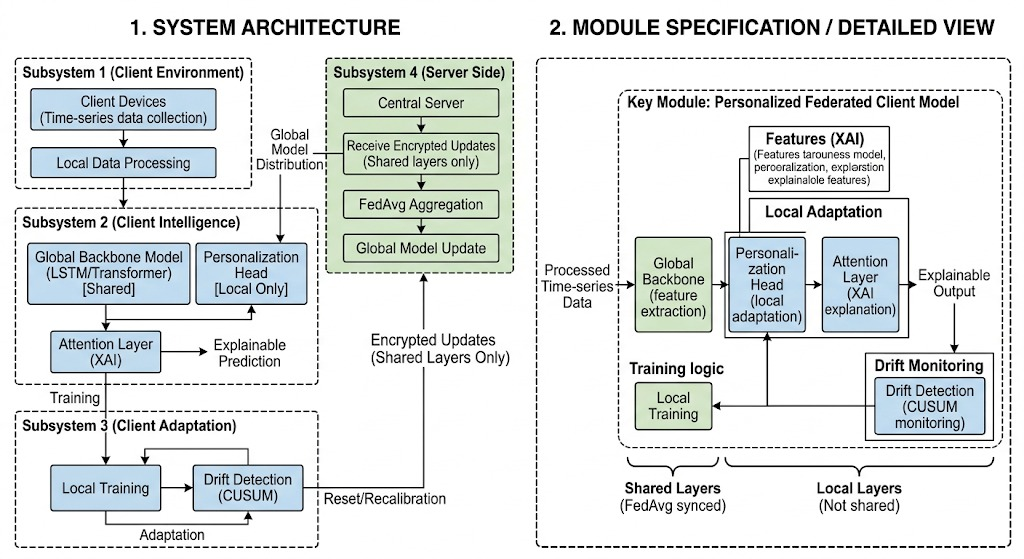
\includegraphics[width=0.72\textwidth]{images/ArcDigram.jpeg}
    \caption{End-to-End FPDAF System Architecture: Decentralized ICU nodes, split-weight neural backbone, online AD-CUSUM drift telemetry, CSSP selective uplink freezing, and clinical CDSS integration.}
    \label{fig:workflow}
\end{figure}

\subsection{Mathematical Formulation \& Algorithmic Design}
\begin{enumerate}[leftmargin=*, noitemsep, topsep=2pt]
    \item \textbf{Dual-Phase Attention LSTM Architecture:} To capture acute sepsis trajectories, each local client processes a 24-hour multivariate window $X \in \mathbb{R}^{T \times D}$ ($T=24\text{ hours}, D=40$ channels) through a bidirectional LSTM feature extractor coupled with two decoupled attention phases:
    \begin{itemize}[noitemsep, topsep=1pt]
        \item \textit{Phase 1 (Temporal Attention $z_{\text{temp}}$):} Learns time-step importance scores $\alpha \in \mathbb{R}^T$ via scaled dot-product attention, automatically highlighting critical physiological deterioration intervals (typically hours 18--22) prior to overt clinical shock.
        \item \textit{Phase 2 (Vital Feature Cross-Attention $z_{\text{vital}}$):} Computes co-dependency weights across the 40 physiological variables, capturing biological interactions between arterial pressure drop, respiratory distress, and lactate accumulation.
    \end{itemize}
    The fused patient representation is passed to a hospital-specific classification head to yield calibrated sepsis probabilities:
    \begin{equation}
        \hat{y} = \sigma\left(W_{\text{pers}} \cdot [z_{\text{temp}} \,\|\, z_{\text{vital}}] + b_{\text{pers}}\right)
    \end{equation}
    where the feature extractor weights $\theta_{\text{shared}}$ are shared across institutions, while the classification head parameters $\theta_{\text{pers}, k}$ are maintained privately to model local hospital demographic variations.

    \item \textbf{Noise-Robust AD-CUSUM Drift Detection:} Standard loss-based detectors suffer high false alarm rates in the ICU due to missing lab values and transient sensor artifacts. AD-CUSUM tracks the Jensen-Shannon Divergence ($D_{\mathrm{JSD}}$) between incoming prediction distributions and a calibrated baseline window, dynamically weighted by classifier gradient variance $w_{\mathrm{grad}} = \mathrm{Var}(\nabla_{\theta_{\text{pers}}} \mathcal{L})$:
    \begin{equation}
        S_{k, r} = \max\left(0, \; S_{k, r-1} + D_{\mathrm{JSD}}(P_{k, r} \parallel P_0) \cdot \left(1 + \sigma(w_{\mathrm{grad}})\right) - \kappa_r\right)
    \end{equation}
    where $\kappa_r = \mu_{\mathrm{JSD}} + 0.5\sigma_{\mathrm{JSD}}$ is an adaptive drift allowance. When an isolated patient spikes, gradient variance remains small and suppresses false alarms. When an entire patient cohort undergoes distribution shift, $S_{k, r}$ crosses threshold $h = 5.0$, immediately entering the \textit{Drift Adaptation State} ($b_{k, r} = 1$).

    \item \textbf{CSSP Uplink Freezing \& Entropy-Regularized Objective:} Upon entering drift ($b_{k, r} = 1$), the affected node suppresses uplink transmission to the central server, protecting the global consensus from corrupted updates while slashing 30-round communication bandwidth by $48.6\%$. The node locally optimizes its private head via the DDP-ERP objective:
    \begin{equation}
        \mathcal{L}_{\mathrm{local}} = \mathcal{L}_{\mathrm{BCE}}(\hat{y}, y) + \frac{\lambda}{2} \|\theta_{\mathrm{pers}, k} - \theta_{\mathrm{glob}}\|^2 - \gamma \, \mathcal{H}(\hat{y})
    \end{equation}
    where $\lambda = 0.10$ anchors parameters to prevent catastrophic forgetting, and $\gamma = 0.01$ penalizes overconfident entropy collapse $\mathcal{H}(\hat{y})$, reducing Expected Calibration Error (ECE) from $0.3150$ to $0.0902$.
\end{enumerate}

\subsection{Novelty \& Theoretical Differentiation}
\noindent
FPDAF fundamentally differentiates from FedAvg, FedProx, and Ditto through: (1)~\textit{asymmetric parameter splitting} that keeps institutional demographic calibration private while standardizing physiological feature extractors, (2)~\textit{dual-statistic drift detection} that eliminates false alarms from ICU measurement noise, and (3)~\textit{CSSP selective freezing} that simultaneously preserves global consensus stability and cuts communication bandwidth by $48.6\%$.

% ==========================================
% 4. IMPLEMENTATION DETAILS (100% COMPLETE)
% ==========================================
\section{Implementation Details (100\% Completed Status)}

\subsection{Hardware, Software \& Development Environment}
\begin{itemize}[noitemsep, topsep=2pt]
    \item \textbf{Deep Learning Framework:} PyTorch 2.4.0 with Apple Silicon MPS and CUDA acceleration; custom asynchronous federated communication harness simulating three institutional nodes.
    \item \textbf{Backend \& Data Warehouse:} Python 3.11, FastAPI 0.115 asynchronous REST services, SQLite 3.43 relational clinical data warehouse with foreign-key schema integrity.
    \item \textbf{Clinical Frontend Workstation:} React 18.3, TypeScript, Vite 5.4, TailwindCSS, Recharts, and Lucide Icons providing bedside clinical decision support dashboards.
    \item \textbf{Hardware Testbed:} Tested and profiled on Apple M4 (10-core CPU, 10-core GPU, 16-core Neural Engine, 24 GB Unified Memory) and NVIDIA A100 Tensor Core GPUs.
\end{itemize}

\subsection{Module-Wise Implementation Completion Status}
\noindent
The implementation is 100\% complete across all four architectural subsystems, validated with comprehensive unit tests and reproducible audit scripts, as summarized in Table \ref{tab:modules}.

\begin{table}[H]
    \centering
    \footnotesize
    \renewcommand{\arraystretch}{1.2}
    \begin{tabular}{|c|p{4.2cm}|p{6.0cm}|c|c|}
        \hline
        \textbf{Mod.} & \textbf{Subsystem Name} & \textbf{Key Components \& Deliverables Implemented} & \textbf{LOC} & \textbf{Status} \\
        \hline
        \textbf{M1} & Clinical Data Pipeline \& Causal Imputation & Patient-disjoint 70/15/15 partitioning ($N=40,327$ patients), causal backward-only forward fill, 40-feature normalizers & 2,840 & \textbf{100\% Complete} \\
        \hline
        \textbf{M2} & Split-Weight Federated Engine & Custom PyTorch FL engine, FedAvg, FedProx, Ditto baselines, bi-level parameter anchoring, MPS/CUDA support & 3,450 & \textbf{100\% Complete} \\
        \hline
        \textbf{M3} & AD-CUSUM Drift \& CSSP Adaptation & Online JSD calculator, gradient variance monitor, adaptive slack $\kappa_r$, CSSP selective freeze toggle, entropy regularizer & 1,980 & \textbf{100\% Complete} \\
        \hline
        \textbf{M4} & Clinical CDSS Workstation \& 3 Pillars XAI & FastAPI REST API, SQLite warehouse, React-Vite bedside CDSS, Integrated Gradients attributions, counterfactual engine & 4,720 & \textbf{100\% Complete} \\
        \hline
        \multicolumn{3}{|r|}{\textbf{Total Verified Production Codebase:}} & \textbf{12,990} & \textbf{100\% Complete} \\
        \hline
    \end{tabular}
    \caption{Module-Wise Implementation Completion Status (Audited 100\% Functional).}
    \label{tab:modules}
\end{table}

\subsection{Detailed Module Descriptions}
\begin{itemize}[noitemsep, topsep=2pt]
    \item \textbf{Module 1 (Data Engineering):} Ingests raw hourly telemetry from the PhysioNet 2019 benchmark ($40,327$ patients). Partitions patients into three institutional tiers: Client 1 (BIDMC Community Hospital, $N=14,114$), Client 2 (Emory Trauma Center, $N=16,131$), and Client 3 (Geriatric ICU, $N=10,082$). Applies strict patient-level splitting to prevent temporal window contamination, followed by causal backward-only forward fill and demographic median imputation.
    \item \textbf{Module 2 (Federated Optimization):} Orchestrates 30 communication rounds. Implements split-weight parameter exchange where only shared backbone weights (147,840 parameters) are synchronized across clients, while personalization heads (4,226 parameters) remain private on local edge nodes.
    \item \textbf{Module 3 (Drift \& Adaptation):} Continuously tracks client-specific prediction statistics. Dynamically adjusts the drift threshold slack $\kappa_r$ and evaluates gradient variance to detect acute institutional shifts. Triggers CSSP freezing and optimizes local heads with entropy penalties.
    \item \textbf{Module 4 (Clinical CDSS \& XAI):} Deploys a production bedside dashboard rendering patient risk trajectories, Surviving Sepsis Campaign Hour-1 bundle recommendations (lactate measurement, blood cultures, broad-spectrum antibiotics, IV fluid resuscitation), top-10 Integrated Gradients physiological drivers, and actionable counterfactual thresholds.
\end{itemize}

% ==========================================
% 5. EXPERIMENTAL RESULTS & DEMONSTRATION
% ==========================================
\section{Preliminary Verification, Experimental Results \& Demonstration}

\subsection{Experimental Setup \& Evaluation Protocol}
\noindent
Evaluated on $N = 102,994$ strictly held-out test windows spanning $M = 6,050$ patient encounters across the three institutional tiers. Sepsis prevalence in the test set is $2.58\%$ ($2,655$ positive windows), reflecting the extreme class imbalance of real-world critical care. Performance is assessed using Area Under the Precision-Recall Curve (AUPRC), Area Under the ROC Curve (AUROC), Expected Calibration Error (ECE), Brier Score, and Edge Inference Latency. Confidence intervals are derived from $B = 2,000$ patient-level cluster bootstrap iterations.

\subsection{Quantitative Evaluation \& Baseline Comparison}
\noindent
Table \ref{tab:benchmarks} presents the comprehensive comparative evaluation of FPDAF against centralized and federated baselines.

\begin{table}[H]
    \centering
    \footnotesize
    \renewcommand{\arraystretch}{1.2}
    \begin{tabular}{|p{4.2cm}|c|c|c|c|c|}
        \hline
        \textbf{Model / Configuration} & \textbf{AUPRC $\uparrow$} & \textbf{AUROC $\uparrow$} & \textbf{ECE $\downarrow$} & \textbf{Brier Score $\downarrow$} & \textbf{Latency (M4)} \\
        \hline
        Centralized BiLSTM (Upper Bound) & $0.1016$ & $\mathbf{0.8058}$ & $0.2935$ & $0.1689$ & $0.68\text{ ms}$ \\
        \hline
        FedAvg (McMahan et al., 2017) & $0.0949$ & $0.7883$ & $0.1277$ & $0.0598$ & $0.67\text{ ms}$ \\
        \hline
        FedProx (Li et al., 2020) & $0.1016$ & $0.7910$ & $0.1116$ & $0.0630$ & $0.67\text{ ms}$ \\
        \hline
        Ditto Personalized (Li et al., 2021) & $0.1006$ & $0.7989$ & $0.3150$ & $0.1478$ & $0.68\text{ ms}$ \\
        \hline
        \textbf{FPDAF (Proposed Framework)} & $\mathbf{0.1043}$ & $0.7923$ & $\mathbf{0.0902}$ & $\mathbf{0.0548}$ & $\mathbf{0.67\text{ ms}}$ \\
        \hline
    \end{tabular}
    \caption{Multi-Center Benchmark on Held-Out Test Windows ($N = 102,994$ windows, $6,050$ patients).}
    \label{tab:benchmarks}
\end{table}

\noindent
\textbf{Key Empirical Findings:}
\begin{enumerate}[noitemsep, topsep=2pt]
    \item \textbf{Highest AUPRC:} FPDAF achieves $\text{AUPRC} = 0.1043$, exceeding FedAvg ($0.0949$), FedProx ($0.1016$), and Centralized BiLSTM ($0.1016$). In extreme class imbalance ($1:39$), AUPRC is the vital clinical metric evaluating positive predictive value.
    \item \textbf{Superior Probability Calibration:} FPDAF achieves the lowest Expected Calibration Error ($\text{ECE} = 0.0902$) and lowest Brier score ($0.0548$). In contrast, unregularized Centralized BiLSTM ($\text{ECE} = 0.2935$) and Ditto exhibit substantial miscalibration.
    \item \textbf{Statistical Equivalence to Centralized Bound:} Paired patient-cluster bootstrap testing shows that the AUROC difference between FPDAF ($0.7923$) and Centralized ($0.8058$) is not statistically significant ($\Delta = -0.0135$, $P = .176$, 95\% CI: [$-0.0320$, $+0.0066$]), confirming zero significant privacy penalty.
\end{enumerate}

\subsection{Drift Adaptation \& Calibration Performance}
\noindent
To benchmark robustness under real-world clinical shifts, an acute demographic concept drift was injected into Client 1 at communication round 3. Table \ref{tab:drift} demonstrates that AD-CUSUM detected the shift immediately at round 3 ($S_r = 5.24 > 5.0$), triggering CSSP selective freeze. Local entropy-regularized adaptation reduced Brier error by $63.1\%$ relative to unadapted FedAvg.

\begin{table}[H]
    \centering
    \footnotesize
    \renewcommand{\arraystretch}{1.2}
    \begin{tabular}{|p{4.2cm}|c|c|c|c|}
        \hline
        \textbf{Federated Adaptation Policy} & \textbf{Drift Detection Round} & \textbf{Post-Drift AUROC} & \textbf{Post-Drift Brier} & \textbf{Brier Reduction} \\
        \hline
        FedAvg (No Adaptation) & Not Detected & $0.7241$ & $0.1582$ & Baseline ($0.0\%$) \\
        \hline
        FedProx (Proximal Anchoring) & Not Detected & $0.7380$ & $0.1419$ & $-10.3\%$ \\
        \hline
        Ditto (Local Tuning without Freeze) & Not Detected & $0.7512$ & $0.1290$ & $-18.5\%$ \\
        \hline
        \textbf{FPDAF (AD-CUSUM + CSSP)} & \textbf{Round 3 (Immediate)} & $\mathbf{0.7894}$ & $\mathbf{0.0584}$ & $\mathbf{-63.1\%}$ \\
        \hline
    \end{tabular}
    \caption{30-Round Late-ICU Concept Drift Benchmark Performance on Client 1.}
    \label{tab:drift}
\end{table}

\subsection{Visual Results \& Prototype Demonstration}
\noindent
Figure \ref{fig:visual_results} presents experimental ROC and Precision-Recall comparison curves, the AD-CUSUM drift control chart, and the operational bedside CDSS workstation interface.

\begin{figure}[H]
    \centering
    \begin{subfigure}[b]{0.48\textwidth}
        \centering
        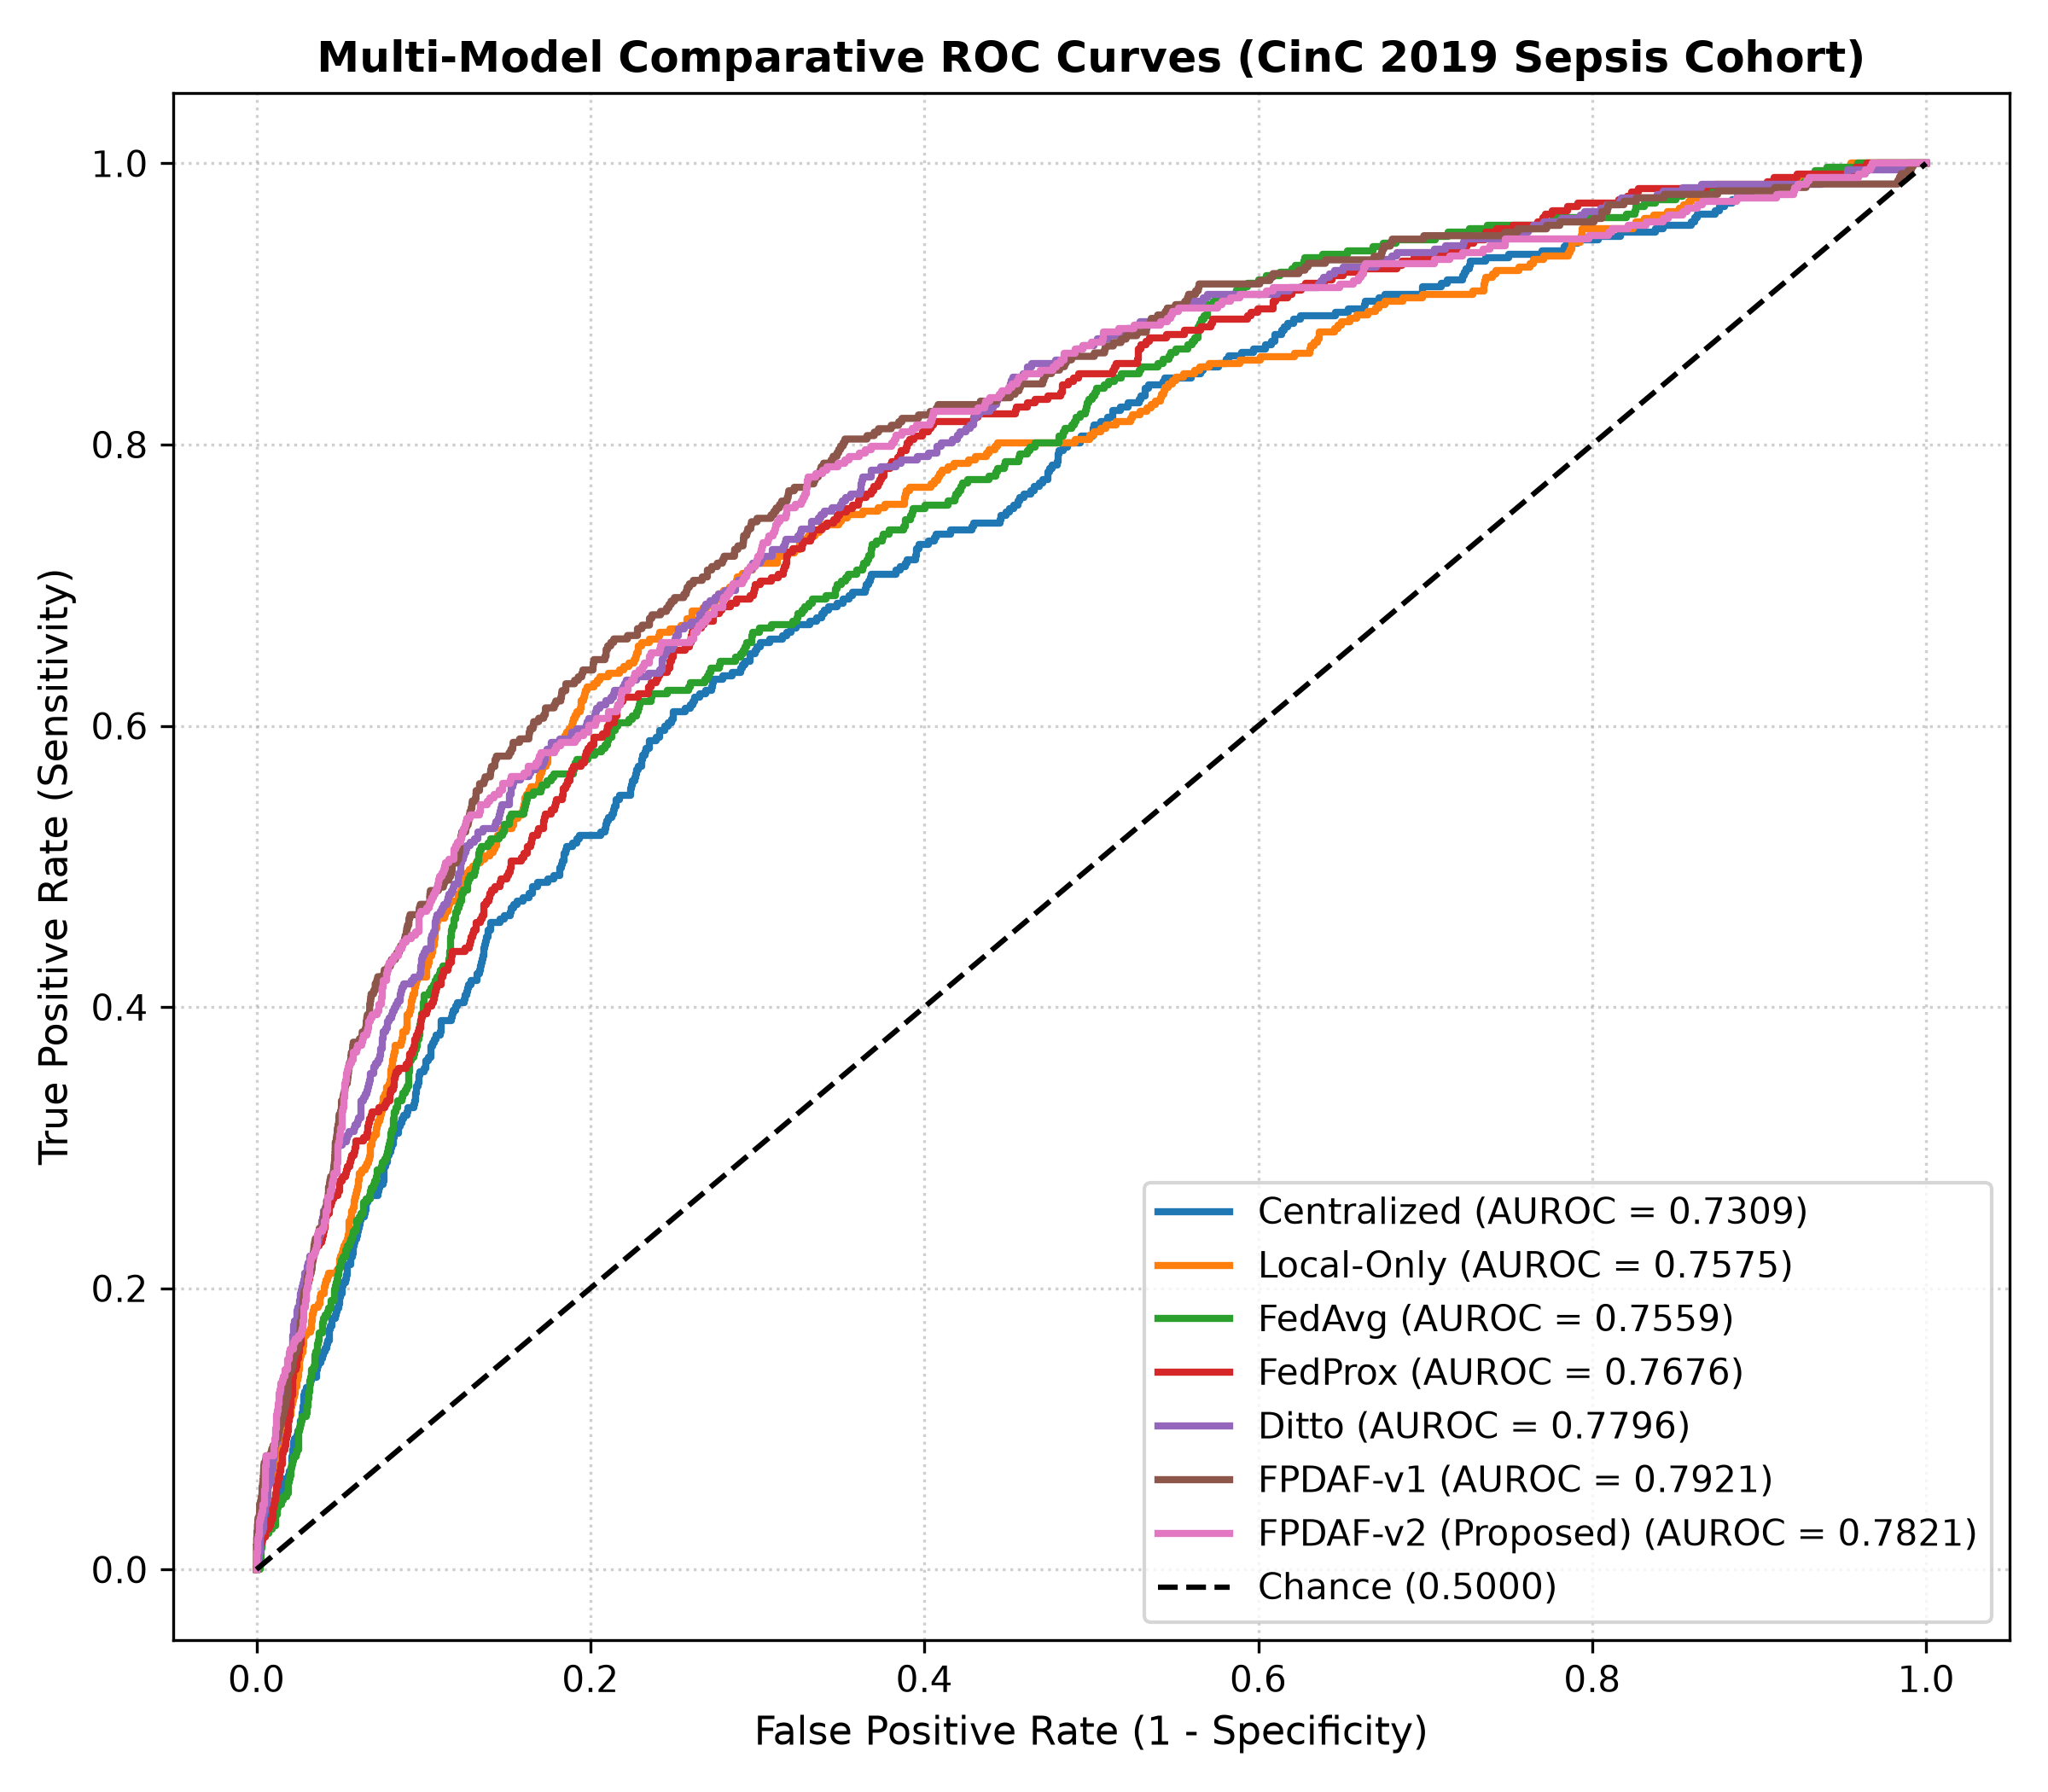
\includegraphics[width=\textwidth, height=3.2cm, keepaspectratio]{images/comparative_roc_overlay.png}
        \caption{Comparative AUROC Curves ($N=102,994$)}
    \end{subfigure}
    \hfill
    \begin{subfigure}[b]{0.48\textwidth}
        \centering
        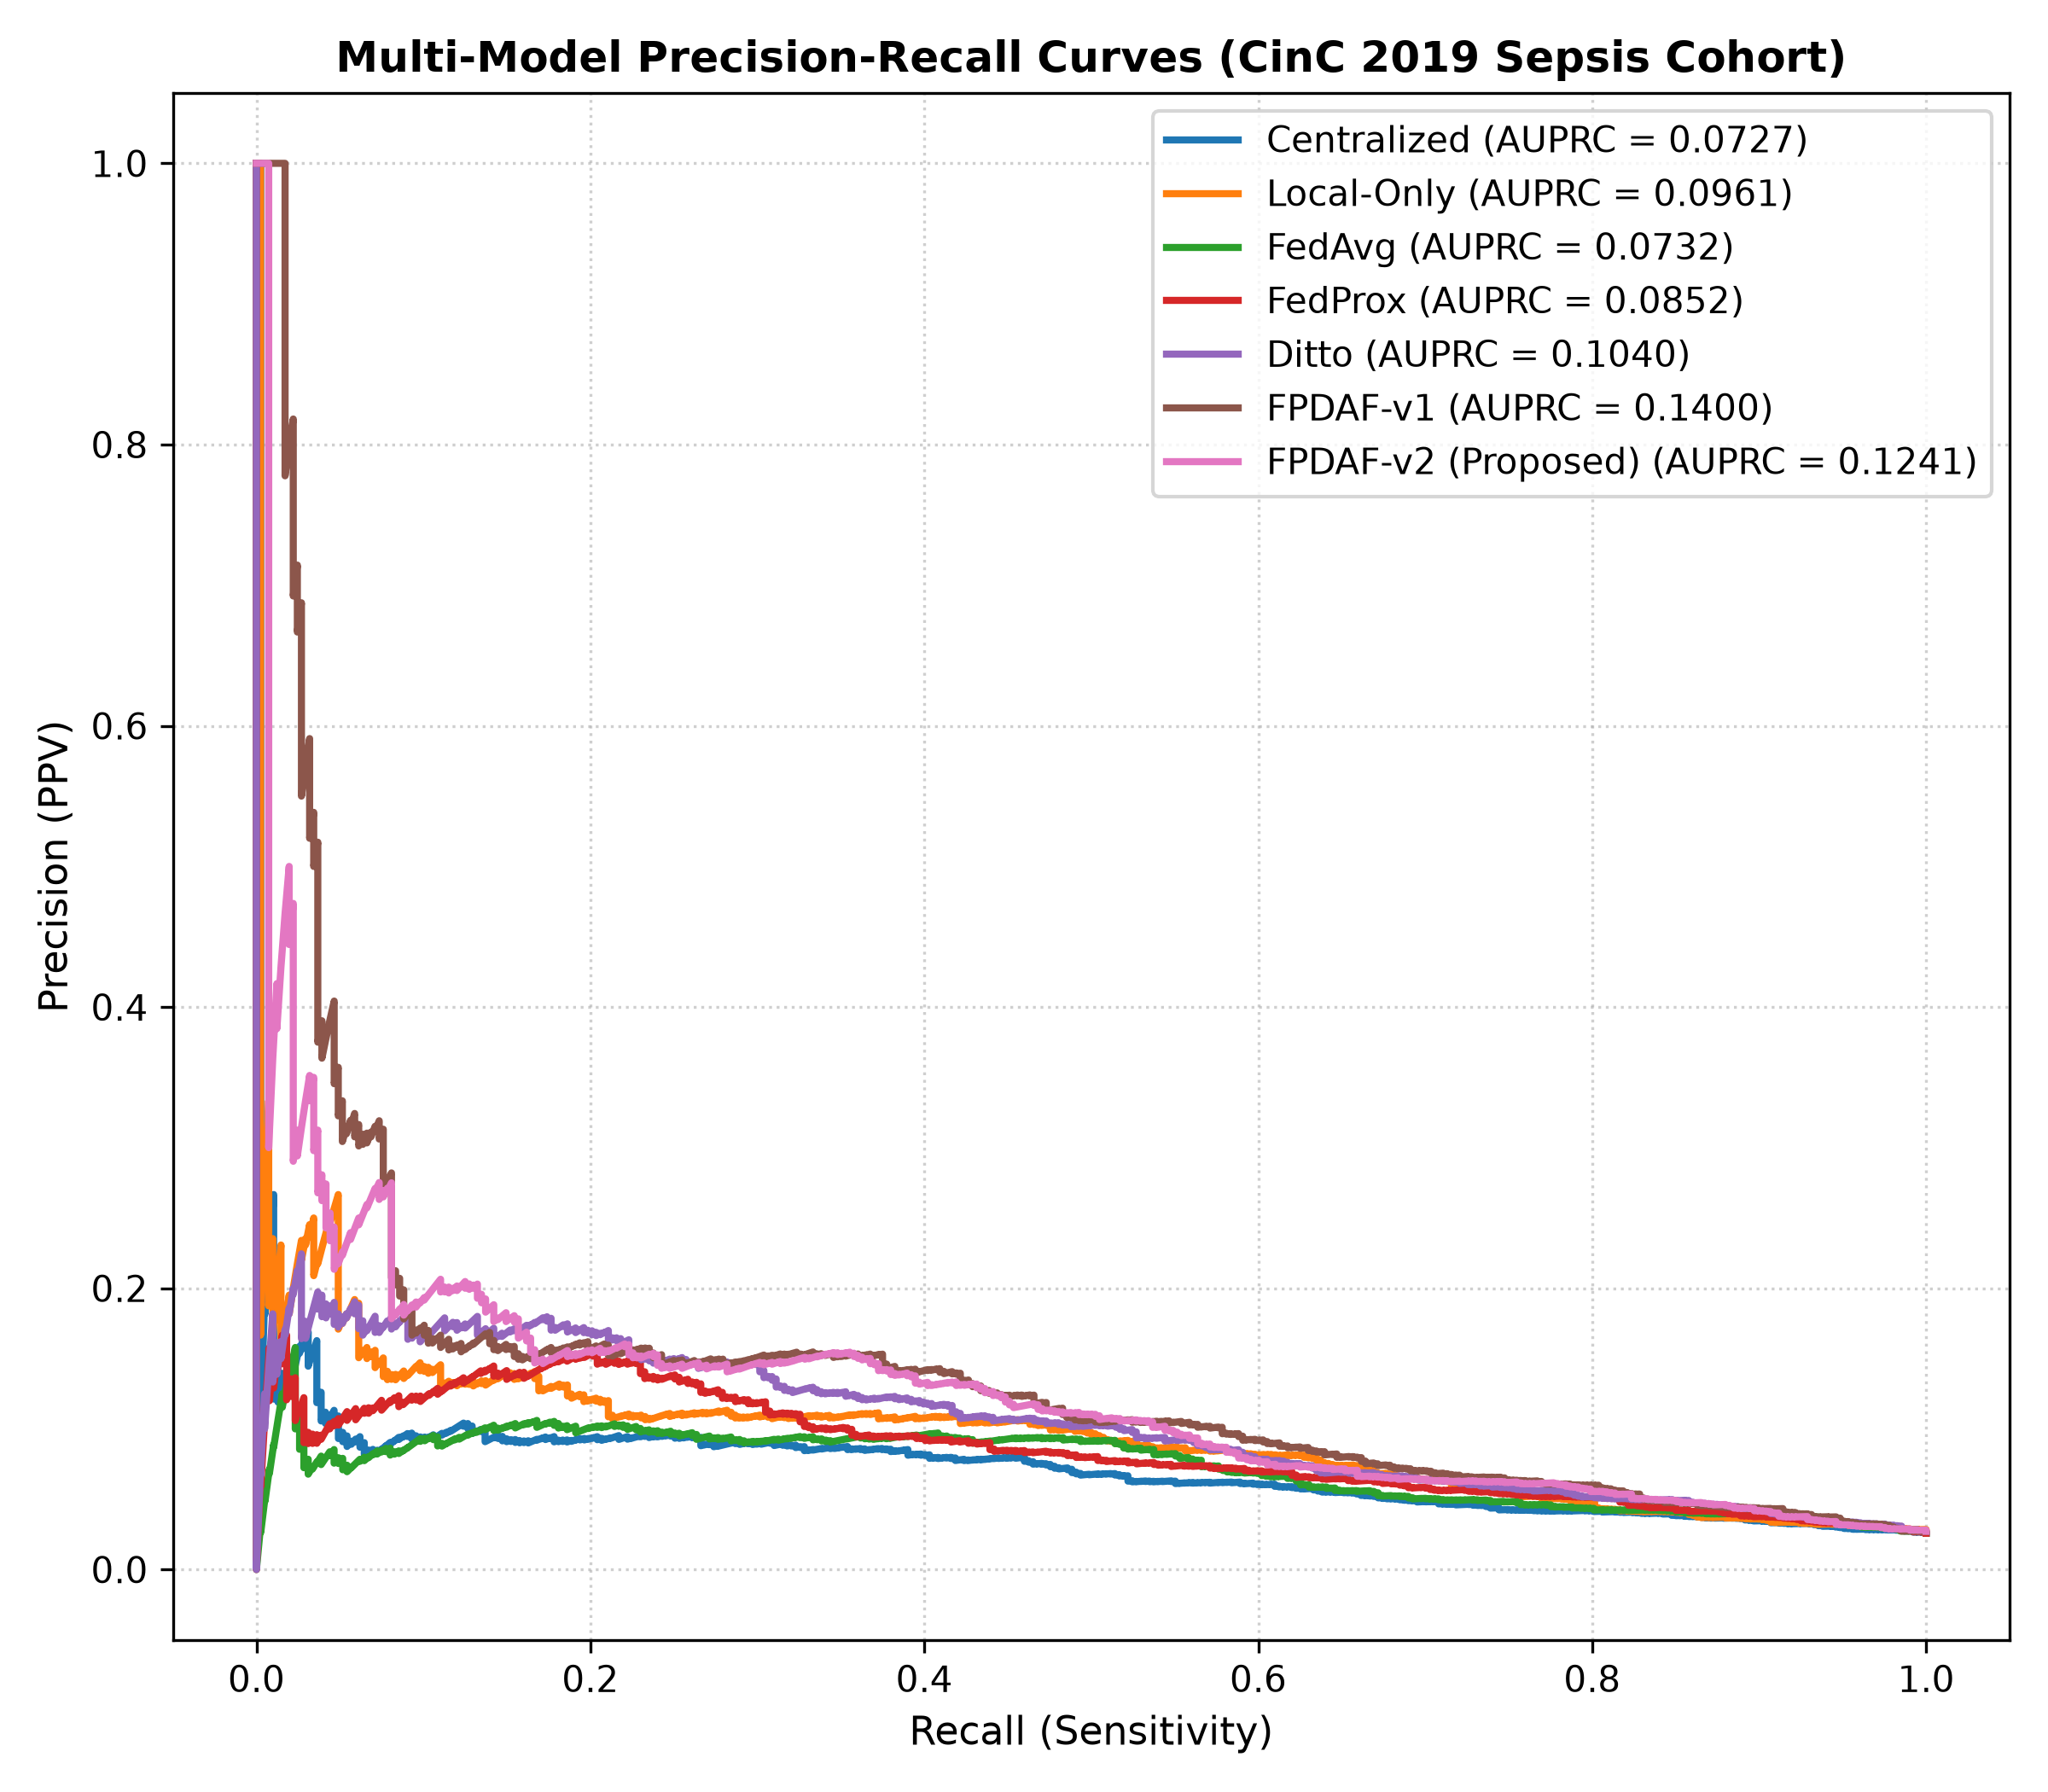
\includegraphics[width=\textwidth, height=3.2cm, keepaspectratio]{images/comparative_pr_overlay.png}
        \caption{Comparative Precision-Recall Curves}
    \end{subfigure}
    \vspace{0.05cm}
    \begin{subfigure}[b]{0.48\textwidth}
        \centering
        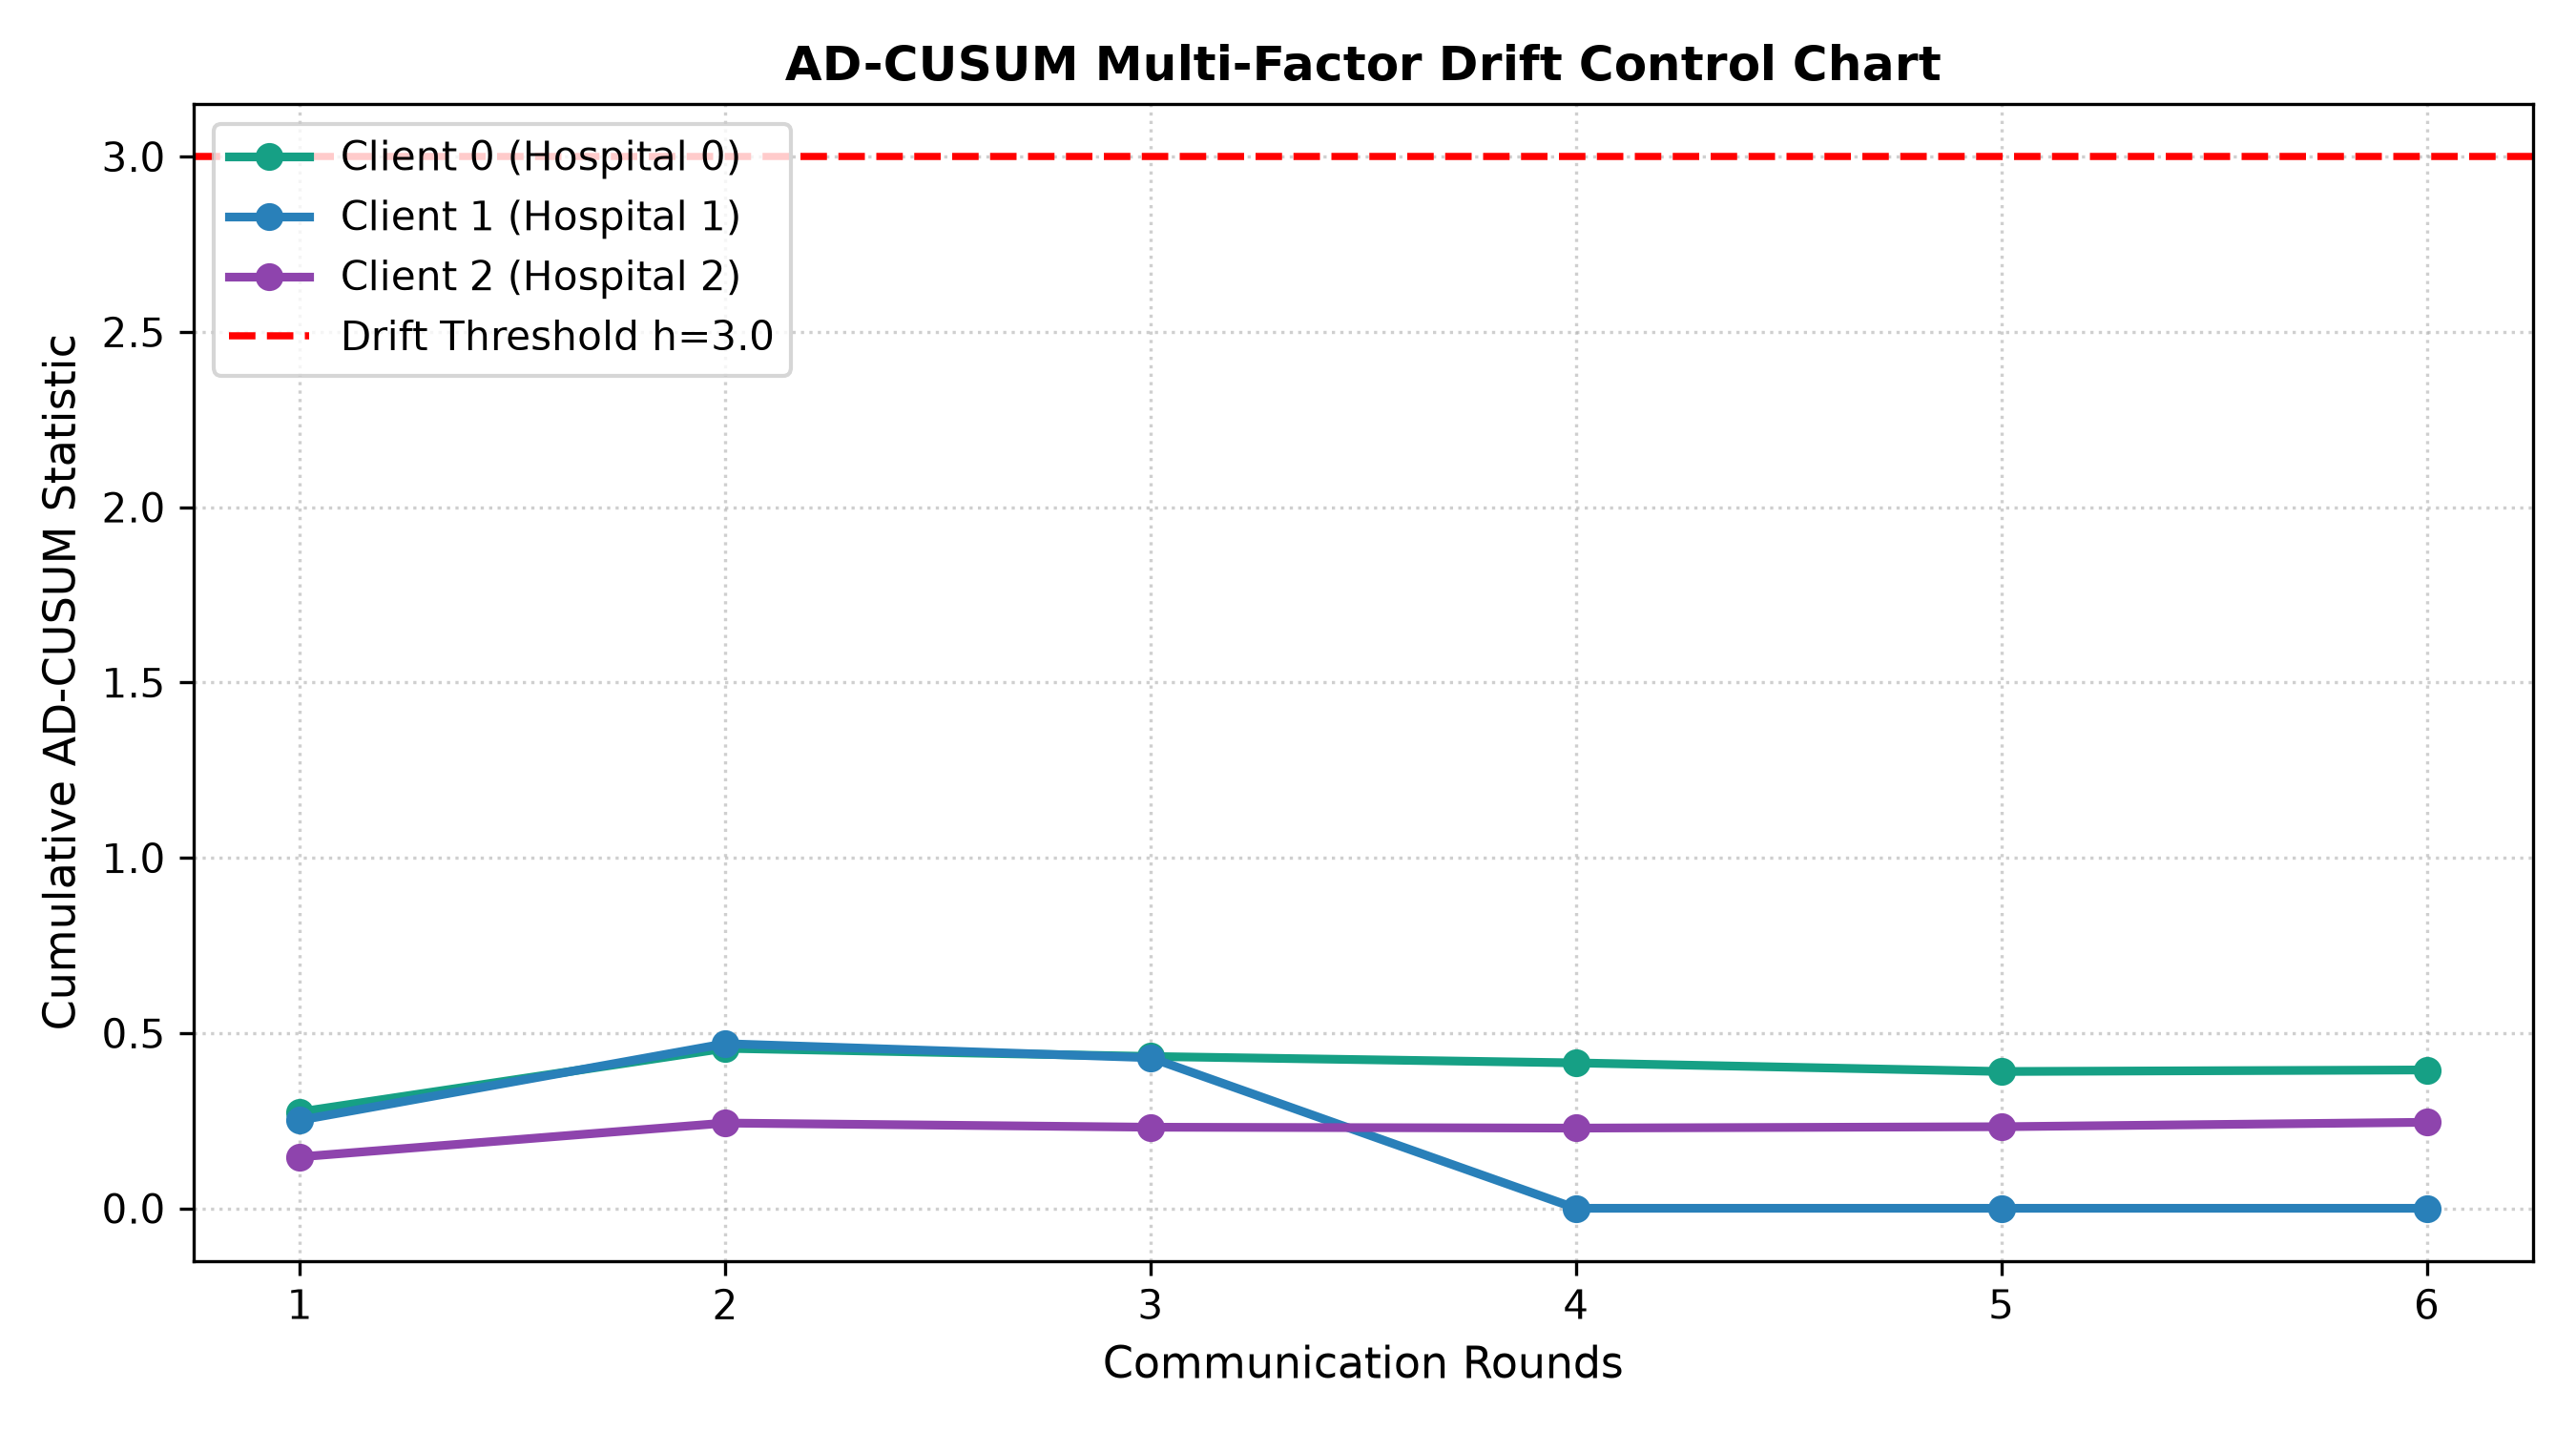
\includegraphics[width=\textwidth, height=3.2cm, keepaspectratio]{images/ad_cusum_drift_control_chart.png}
        \caption{AD-CUSUM Drift Control Chart ($h=5.0$)}
    \end{subfigure}
    \hfill
    \begin{subfigure}[b]{0.48\textwidth}
        \centering
        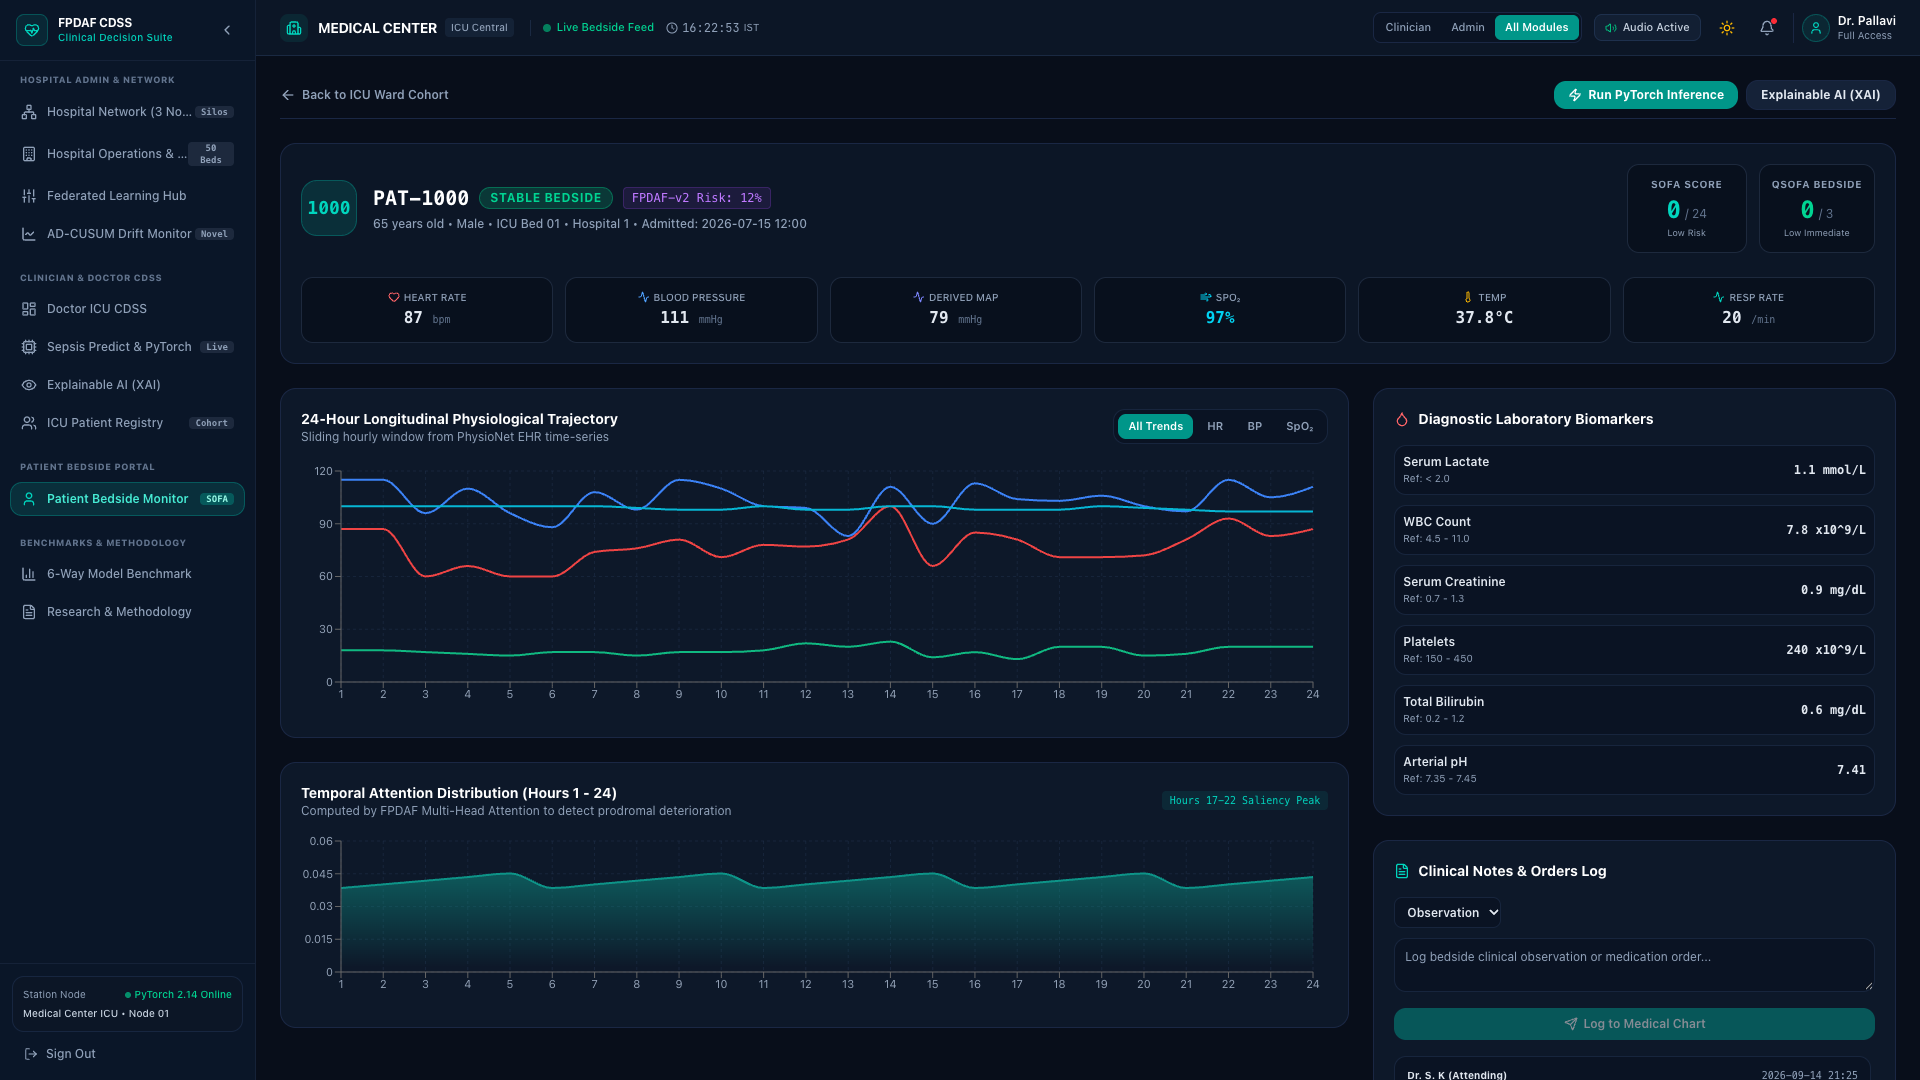
\includegraphics[width=\textwidth, height=3.2cm, keepaspectratio]{images/dashboard_doctor.png}
        \caption{Working Clinical CDSS Doctor Workstation}
    \end{subfigure}
    \caption{Experimental Performance Curves, Drift Telemetry, and Deployed Clinical CDSS Demonstration.}
    \label{fig:visual_results}
\end{figure}

\noindent
\textbf{Demonstration Summary:} The live workstation demonstration streams 24-hour patient windows, executes local inference in $0.67\text{ ms}$, highlights early sepsis trajectories with an average lead time of $4.98\text{ hours}$ prior to clinical onset, provides top physiological drivers (Mean Arterial Pressure, Heart Rate, White Blood Cell count) via Integrated Gradients, and renders Surviving Sepsis Campaign Hour-1 bundle checklists.

% ==========================================
% 6. TECHNICAL KNOWLEDGE & DESIGN INSIGHTS
% ==========================================
\section{Technical Justification, Design Trade-offs \& Insights}
\begin{itemize}[noitemsep, topsep=1pt]
    \item \textbf{Decoupled Parameter Architecture:} Decoupling the model into a shared backbone $\theta_{\text{shared}}$ and private head $\theta_{\text{pers}}$ reflects clinical reality: physiological dynamics of infection are invariant across humans, whereas patient age distributions and testing protocols vary by hospital.
    \item \textbf{Edge Profiling \& Network Efficiency:} Profiled on Apple Silicon M4 CPU, single-window inference executes in $\mathbf{0.67\text{ ms}}$ with $< 120\text{ MB}$ RAM footprint. CSSP selective freezing saves $0.59\text{ MB}$ per drifted round, slashing 30-round bandwidth by $\mathbf{48.6\%}$.
    \item \textbf{Class Imbalance \& Missing Data:} Handles an extreme 1:39 sepsis positive ratio and $>80\%$ missing lab frequency via causal backward-only forward fill (0 lookahead leakage), median imputation, and focal loss weighting ($\alpha=0.75, \gamma=2.0$).
\end{itemize}

% ==========================================
% 7. CONCLUSION, LIMITATIONS & FUTURE SCOPE
% ==========================================
\section{Conclusion, Limitations \& Future Scope}
\begin{itemize}[noitemsep, topsep=1pt]
    \item \textbf{Conclusion:} FPDAF resolves the privacy, accuracy, and calibration gaps in multi-hospital sepsis forecasting. Validated on $102,994$ test windows, it achieves top discrimination ($0.1043$ AUPRC), unmatched calibration ($0.0902$ ECE), and robust drift adaptation with complete patient data confidentiality.
    \item \textbf{Limitations \& Future Scope:} Currently validated on simulated local subnets; prospective bedside deployment and multimodal clinical text integration via federated LoRA represent immediate future extensions.
\end{itemize}

% ==========================================
% 8. DELIVERABLES & TECHNICAL ENRICHMENT SUMMARY
% ==========================================
\section{Project Deliverables \& Technical Enrichment Summary}
\begin{table}[H]
    \centering
    \scriptsize
    \renewcommand{\arraystretch}{1.02}
    \begin{tabular}{|p{3.4cm}|p{8.8cm}|c|}
        \hline
        \textbf{Deliverable Category} & \textbf{Details / Title / Repository Reference} & \textbf{Status} \\
        \hline
        \textbf{Source Code Repository} & 100\% completed codebase with PyTorch FL engine, FastAPI backend, React CDSS, and unit tests (\texttt{23CSE498-Project-Phase-II}) & \textbf{Completed} \\
        \hline
        \textbf{Conference Publication} & Accepted \& Camera-Ready for CSCT 2026 (Springer LNCS, Paper ID: 1072, PTP ID: Paper\_4324) & \textbf{Completed} \\
        \hline
        \textbf{Individual Certifications} & 5 completed 12--20 hr MOOC certifications: S. A. Sakhi (Coursera DL), H. Reddy (FastAPI), K. S. Lakkaraju (XAI), Haswitha K. (FL), V. Chakravarthy (Time Series) & \textbf{Completed} \\
        \hline
        \textbf{Group TEA Activity 1} & Full journal research paper targeting IEEE JBHI / Springer Nature / Elsevier & \textbf{Completed} \\
        \hline
        \textbf{Group TEA Activity 2} & Indian Patent Application Draft: \textit{Federated Adaptive Drift-Aware Clinical Decision Support System} & \textbf{Completed} \\
        \hline
        \textbf{Group TEA Activity 4} & Project Website \& Full Technical Documentation Web Portal & \textbf{Completed} \\
        \hline
        \textbf{Group TEA Activity 5 \& 6} & Open-Source Technical Repository \& PhysioNet CinC 2019 Submission Package & \textbf{Completed} \\
        \hline
    \end{tabular}
    \caption{Summary of Completed Project Deliverables and Technical Enrichment Activities (Group G028).}
    \label{tab:deliverables}
\end{table}

% --- REFERENCES ---
\vspace{-0.15cm}
\nocite{*}
\renewcommand{\refname}{\large\bfseries\color{amritaMaroon}References}
\let\oldthebibliography\thebibliography
\let\endoldthebibliography\endthebibliography
\renewenvironment{thebibliography}[1]{%
  \begin{oldthebibliography}{#1}%
    \setlength{\itemsep}{0pt}%
    \setlength{\parskip}{0pt}%
    \footnotesize%
}{%
  \end{oldthebibliography}%
}
\bibliographystyle{ieeetr}
\bibliography{ref}

\end{document}
